\chapter{Stereolithography \texttt{.stl} files}

\verb|.stl| is a file format which dates back to $1987$ when it has been created by \textit{$3$D Systems}\footnote{American company that engineers, manufactures and sells $3$D printers, $3$D printing materials, $3$D printed parts and application engineering services. For further information we refer to~\url{https://www.3dsystems.com/}} for its stereolithography (from which the file extension originates) printing technology for commercial $3$D printers. Eventually it became the $3$D printing and rapid prototyping industry's defacto standard. In general \verb|.stl| files are also referred to as standard triangle language or standard tessellation language files.

\smallskip
The \verb|.stl| format is used to describe an unstructured triangulated surface using a list of triangles. Each of these triangles is described separately by its own normal and  vertices using a Cartesian coordinate system~\cite{wiki:stl_file_format}. Their main purpose is to describe the surface geometry of a $3$D object, thus in this files, differently from CAD files, no information about colors or textures is present. They also do not contain any scale information and can be specified both in ASCII and binary representation.

\smallskip
An example of of a \verb|.stl| file in ASCII format is:
\begin{verbatim}
solid topFace
    facet normal -0.000000e+00  0.000000e+00  1.000000e+00
        outer loop
            vertex   0.000000e+00 -0.000000e+00  5.000000e-01
            vertex   5.000001e-02 -5.000001e-02  5.000000e-01
            vertex   5.000001e-02 -0.000000e+00  5.000000e-01
    endloop
endfacet
...
endsolid topFace
solid fixedFaces
    facet normal  0.000000e+00  1.000000e+00  0.000000e+00
        outer loop
            vertex   0.000000e+00 -0.000000e+00  0.000000e+00
            vertex   5.000001e-02 -0.000000e+00  5.000000e-02
            vertex   5.000001e-02 -0.000000e+00  0.000000e+00
        endloop
    endfacet
...
endsolid fixedFaces
\end{verbatim}
This is the \verb|.stl| file that we have used to represent the geometry used in the $3$D design optimization problem in section~\vref{sec:results_3D_case}. In the same file showed above are stored two different surfaces named respectively \verb|topFace| and \verb|fixedFaces|; each triangle of a surface is described by means of a \verb|facet| (we reported only one triangle per surface for brevity) which specify its normal and the coordinates of its vertices arranged counterclockwise.
Those files can also be stored in binary format, which is particularly convenient for large files.

\smallskip
We finally remark that, in general, \verb|.stl| files contain only an \emph{approximation} of geometry surfaces. An example of this situation can be found in figure~\vref{fig:sphere_real_and_meshed}, specifically in figure~\ref{subfig:sphere_meshed} it can be seen how the red lines of the triangle edges are not capable to perfectly reconstruct the smoothness of the original surface (figure~\ref{subfig:sphere_real}). Augmenting the number of triangles of the mesh improve the approximation, at cost of larger \verb|.stl| files, but will not be possible to perfectly reconstruct curved surfaces.

\begin{figure}
	\centering
	\subfloat[][\emph{Original sphere}]
	{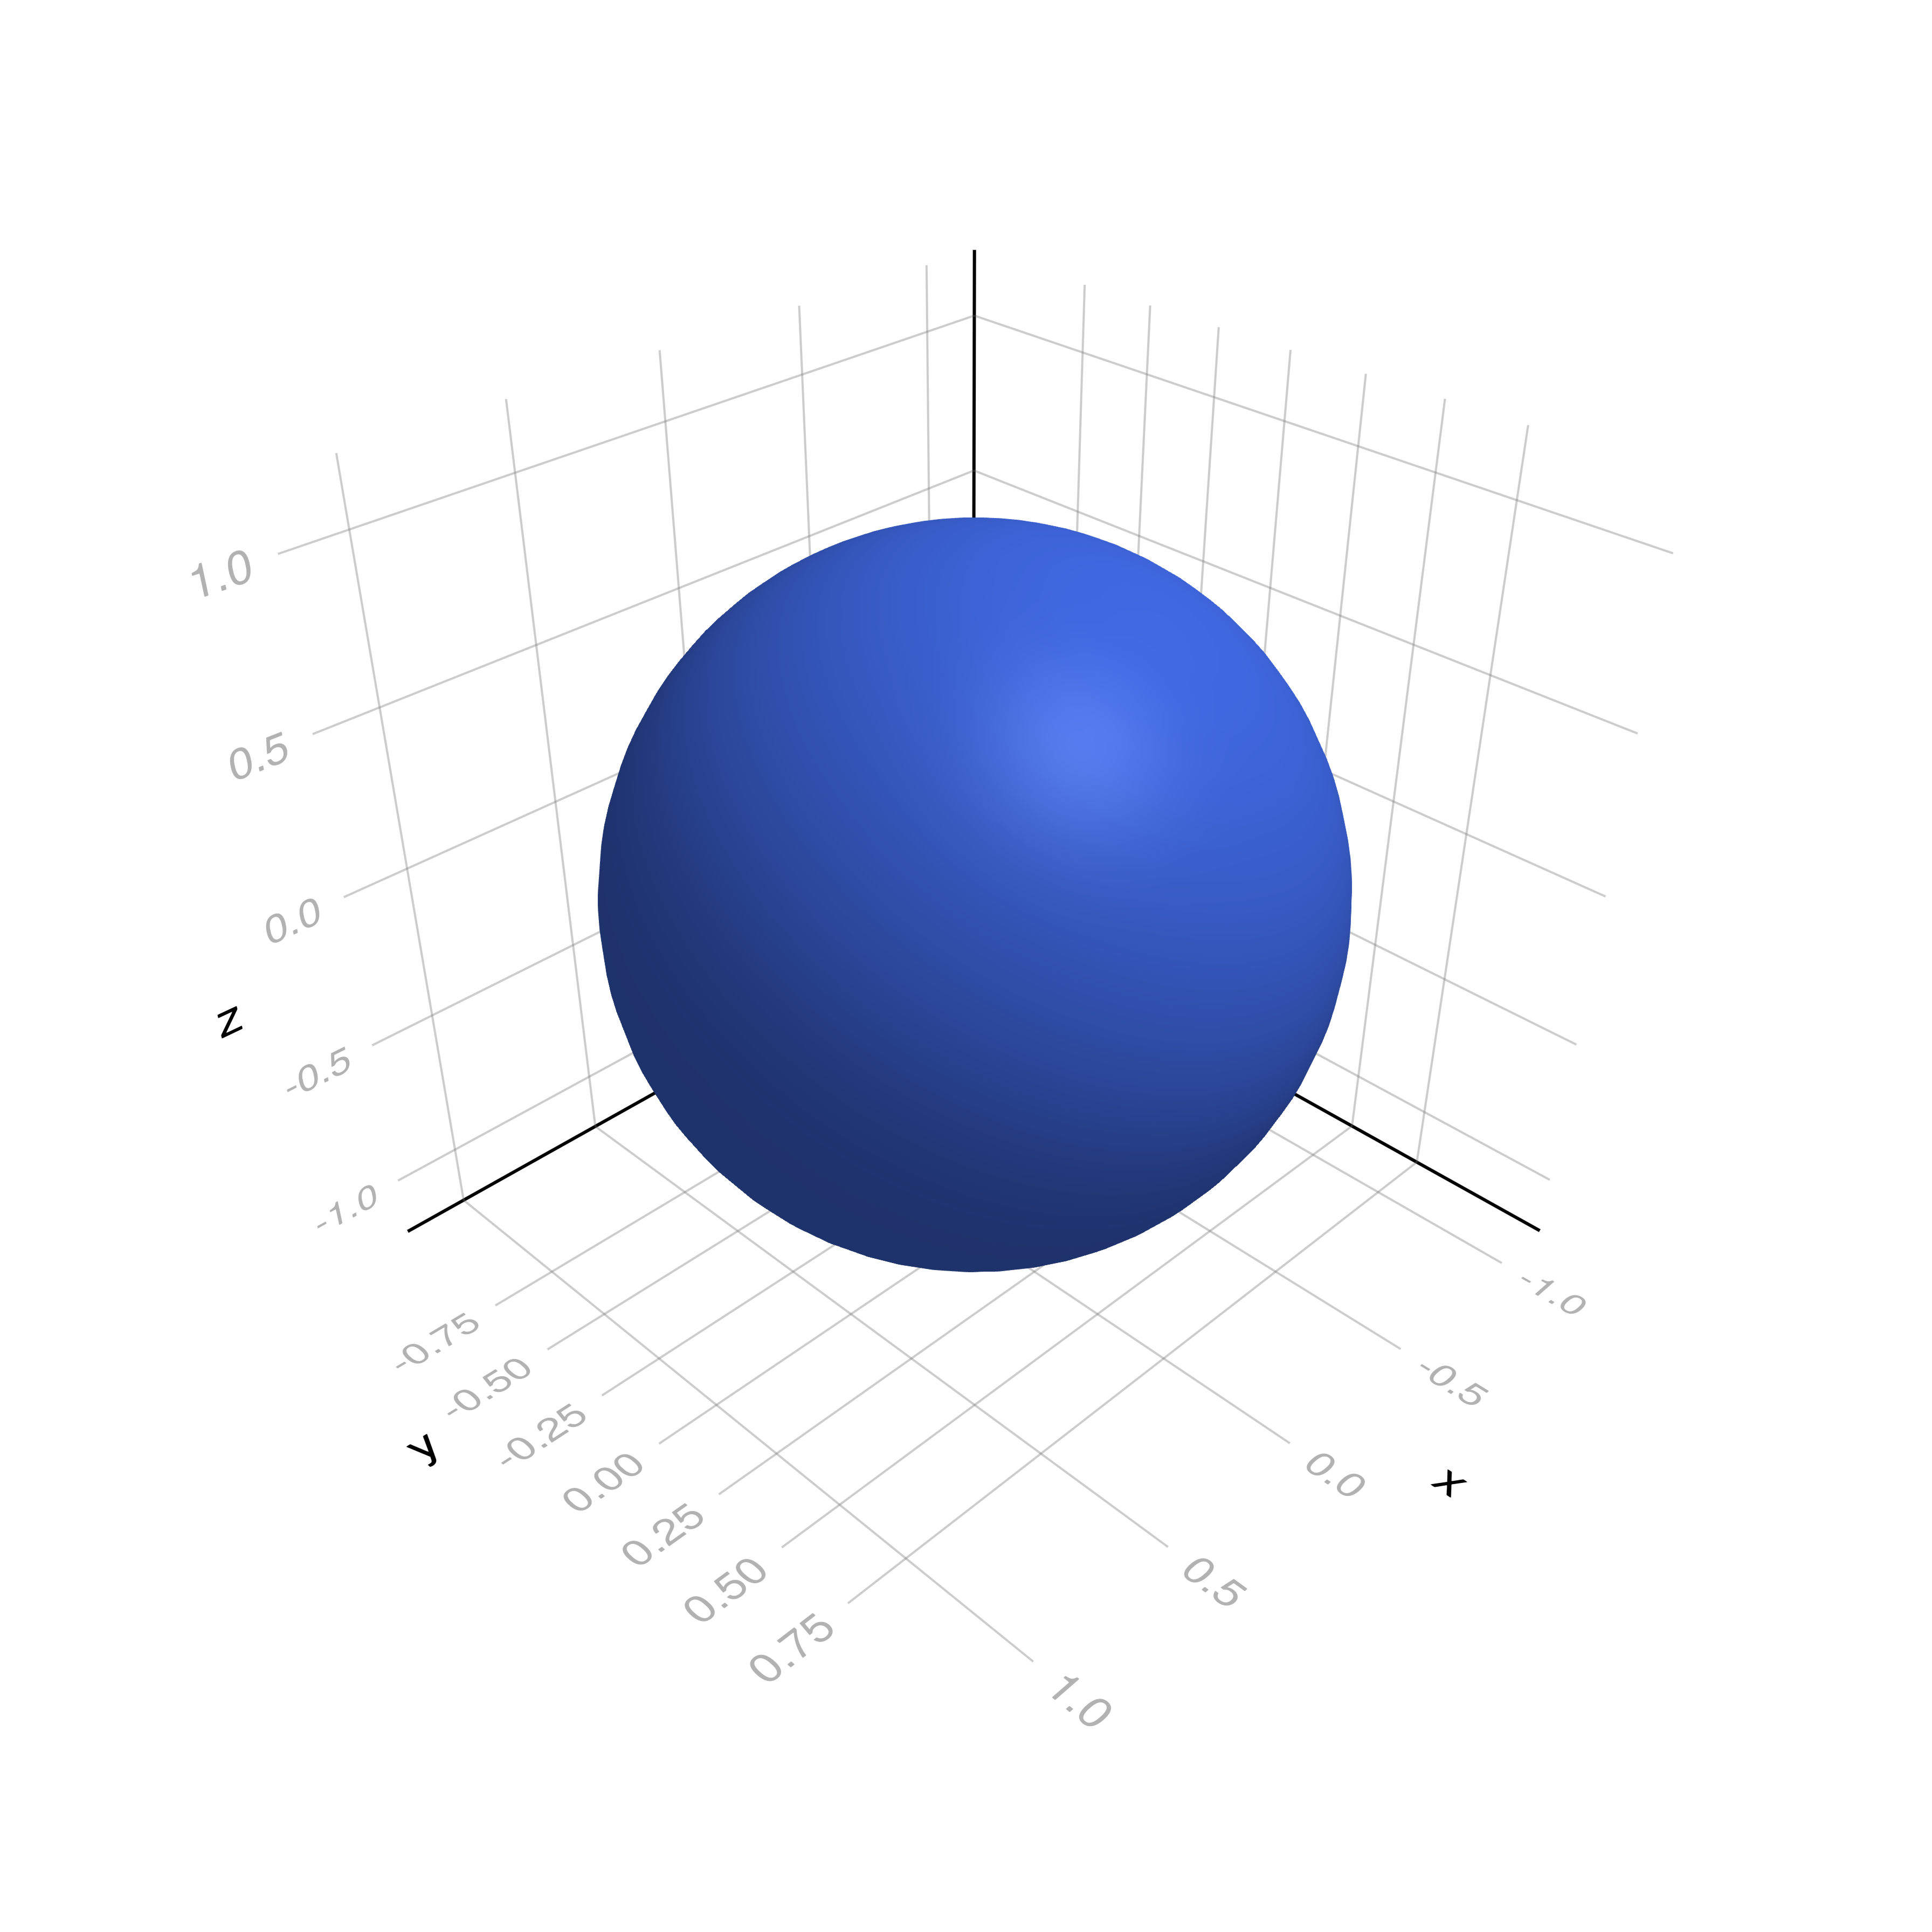
\includegraphics[width=.55\textwidth]{img/sphere_real.png}\label{subfig:sphere_real}} \\
	\subfloat[][\emph{Sphere \texttt{.stl} representation}]
	{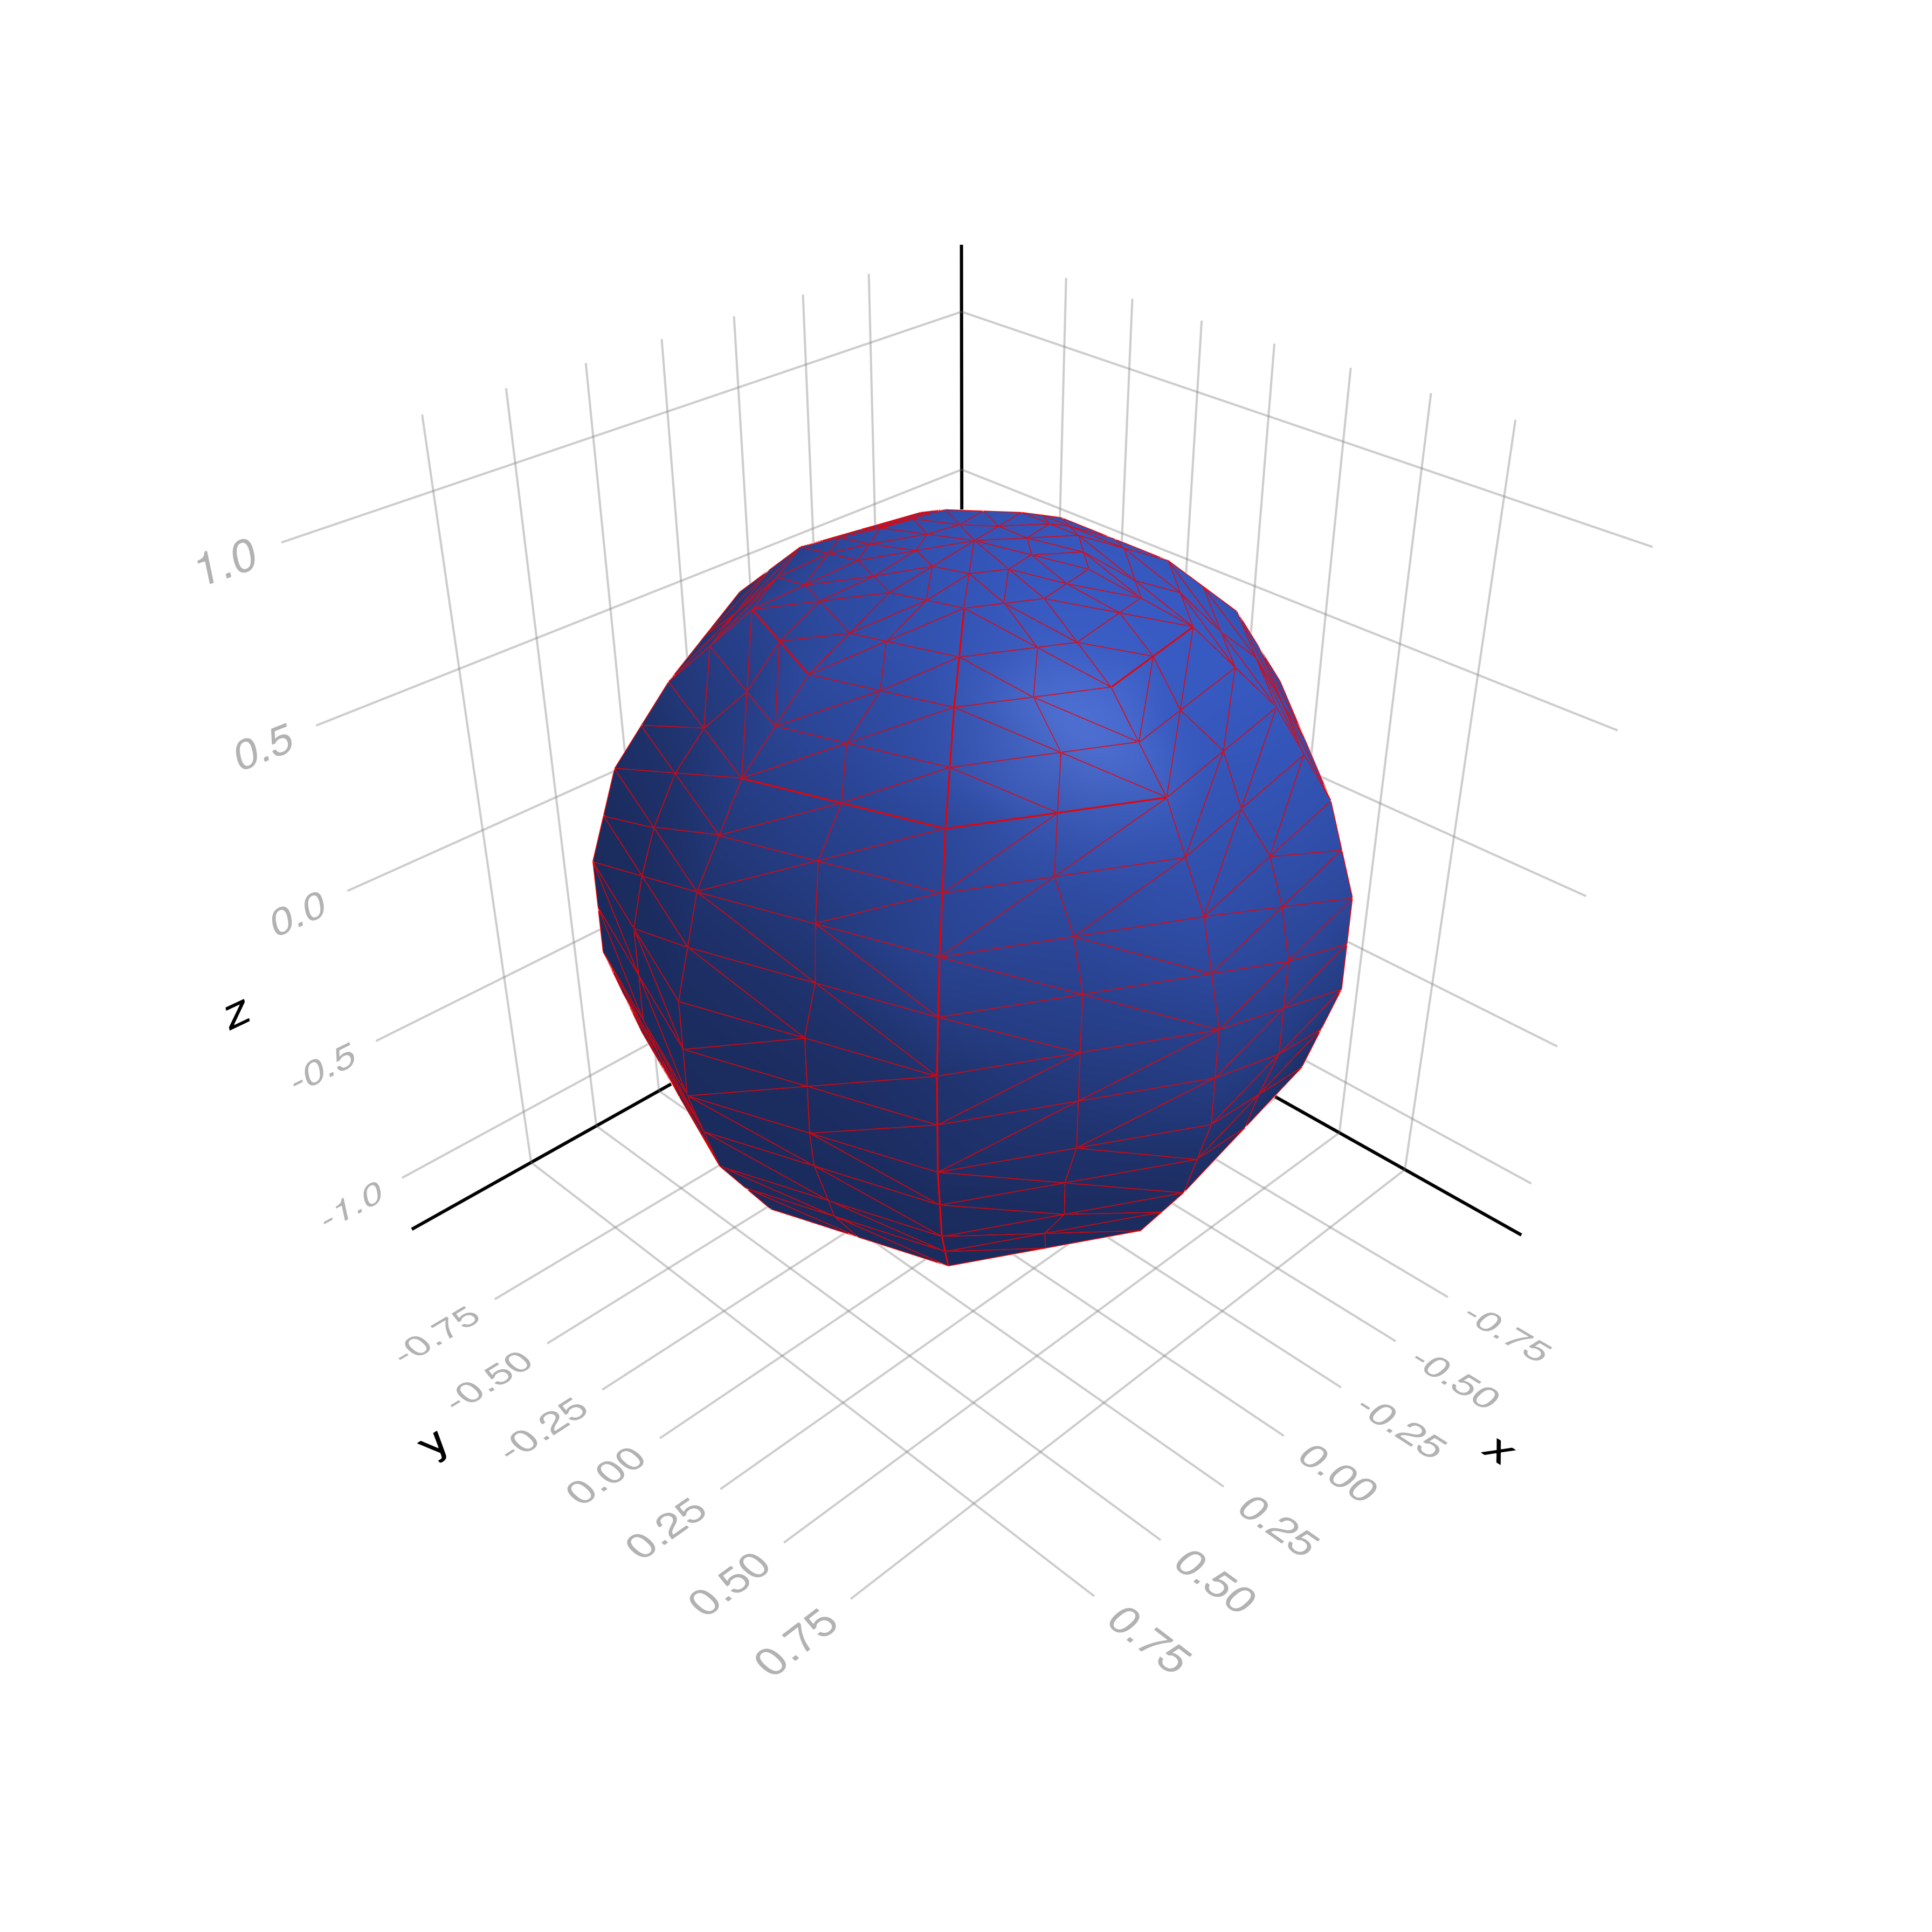
\includegraphics[width=.55\textwidth]{img/sphere_meshed.png}\label{subfig:sphere_meshed}}
	\caption{Example of approximating the surface of a unit-radius sphere centered at the origin using an \texttt{.stl} file}
	\label{fig:sphere_real_and_meshed}
\end{figure}

%TODO: About the history
